\documentclass[prb,9pt,notitlepage]{revtex4-1}
%\documentclass[a4paper,twocolumn,9pt]{article}

%\usepackage{geometry}
%\geometry{a4paper,top=2.5cm,bottom=2cm,inner=1.5cm,outer=1.5cm}

\usepackage{mwe}% just for the example content
\usepackage{color}
\usepackage{latexsym,amsmath}
\usepackage{physics}
\usepackage{listings}
\usepackage[dvipsnames]{xcolor}
\usepackage{parskip}
\usepackage{hyperref}
%\usepackage{dblfloatfix}
%\usepackage{subfig}
\definecolor{linkcolor}{rgb}{0,0,0.65}%hyperlink
\definecolor{shadecolor}{rgb}{0.93, 0.93, 0.93}
%\usepackage[pdftex,colorlinks=true, pdfstartview=FitV, linkcolor= linkcolor, citecolor= linkcolor, urlcolor= linkcolor, hyperindex=true,hyperfigures=true]{hyperref} %hyperlink%
%\usepackage[backend=biber, sorting=ynt]{biblatex}
%\usepackage{ragged2e} % to justify caption
%\addbibresource{bibliography.bib}
 \usepackage{booktabs}

\usepackage[T1]{fontenc}
\usepackage{xcolor}
\usepackage{lmodern}
\usepackage{listings}
\lstset{language=[95]Fortran,
  backgroundcolor=\color{shadecolor},
  basicstyle=\ttfamily,
  keywordstyle=\color{blue},
  commentstyle=\color{gray},
  stringstyle=\color{red},
  showstringspaces=false
  %morecomment=[l]{!\ }% Comment only with space after !
}

\usepackage{tabularx}

\usepackage{fancyhdr}
\pagestyle{fancyplain}% <- use fancyplain instead fancy
\fancyhf{}
\fancyhead[R]{\today}
\fancyhead[L]{Alessandro Lambertini}
\fancyfoot[L]{Quantum information and computing}
\fancyfoot[C]{Report 2}
\fancyfoot[R]{\thepage}

\renewcommand{\headrulewidth}{0pt}

\usepackage{float}
\usepackage{siunitx}




\begin{document}
\title{Quantum information and computing: Exercises report, week 4. \\ Multi-run script \& Automated fits }

\author{Alessandro Lambertini}


\date{\today}

\begin{abstract}
Through the exercise of this week,  we start to tackle the Many-Body Problem. We will try to implement some methods to handle N-body non interacting, separable/non-separable, pure states. We will write the density matrix of a pure state given $N=2$, exploit a subroutine to compute the reduce density matrix of either the left or the right subsystem once a density matrix in $\mathcal{H}^{D^2}$ is given. Finally, we will test all the instruments deleveloped on a system made of two qubits.
\end{abstract}

\maketitle

\section{Theory}
Considering a system made of $N$ particles, each one described by a wavefunction $\psi_i$ living in a d-dimensional Hilbert space $\mathcal{H}^d$, we have that the wavefunction $\Psi$ of the whole system is given by:
\begin{equation}
  \ket{\Psi} = \sum_{\alpha_1,\dots,\alpha_N} C_{\alpha_1,\dots,\alpha_N}\ket{\psi_{\alpha_1}}\otimes\ket{\psi_{\alpha_2}}\otimes \dots\otimes\ket{\psi_{\alpha_N}} \qquad \alpha_j \in \{1,\dots,D\}
\end{equation}

Sometimes we encounter special kind of states, called separable, which can be written as a sum of $N$ pure state over each subsystem. In other words, we call a state separable if we can write it as:
\begin{equation}
  \ket{\Psi} = \sum_{\alpha_1}C_{\alpha_1}\ket{\psi_{\alpha_1}}\otimes\sum_{\alpha_2}C_{\alpha_2}\ket{\psi_{\alpha_2}}\otimes\dots\otimes\sum_{\alpha_N}C_{\alpha_N}\ket{\psi_{\alpha_N}}
\end{equation}
and so describe it with only $dN$ coefficients instead of $d^N$.

Given a generic state $\ket{\Psi}$ the density matrix $\rho$ that describes that state is defined as:
\begin{equation}
  \rho = \ket{\Psi}\bra{\Psi}
\end{equation}
Describing a quantum state by its density matrix is a fully general alternative formalism to describing a quantum state by its state vector (its "ket") or by a statistical ensemble of kets
Given a generic density matrix $\rho$ in $\mathcal{H}^{d^N}$ , the reduced density matrix relative to the k-subsystem is:
\begin{equation}
  \rho_k = Tr_1\dots Tr_{k-1}Tr_{k+1}\dots Tr_N\rho \qquad \mbox{where} \qquad \Tr_j\rho = \sum_{j=1}^D\bra{j}\rho\ket{j}
\end{equation}


\section{Code development}
In order to describe properly any kind of state separable or not I implemented a derived type in fortran called \textit{pure\_state}
\begin{lstlisting}
type pure_state
  integer(kind=8) :: dim
  integer(kind=8) :: N_particles
  logical :: is_separable
  complex(kind=8), dimension(:), allocatable :: psi
end type

\end{lstlisting}
where it is initialized the dimension of any subsystem, the number of particles our system is made of, a logical variable that controls if the state is separable or not, and a complex arrays that has to be properly initialized to describe the state.
Moreover, I implemented a subroutine useful to allocate properly the memory based on the kind of the state:
\begin{lstlisting}
!!!!!!!!!!!!!!!!!!! allocate the memory for a pure state !!!!!!!!!!!!!!!!!!!
!!!!!!!!!!!!!!!!!!!!!!!!!!!!! separable or not !!!!!!!!!!!!!!!!!!!!!!!!!!!!!
subroutine init_pure_state(state,dim,N,separable)
  type(pure_state) :: state
  integer(kind=8) :: dim
  integer(kind=8) :: N
  logical :: separable

  if ( separable ) then
    state%dim = dim
    state%N_particles = N
    allocate(state%psi(dim*N))
    state%is_separable = .true.
  else
    state%dim = dim
    state%N_particles = N
    allocate(state%psi(dim**N))
    state%is_separable = .false.
  end if
end subroutine init_pure_state
!!!!!!!!!!!!!!!!!!!!!!!!!!!!!!!!!!!!!!!!!!!!!!!!!!!!!!!!!!!!!!!!!!!!!!!!
\end{lstlisting}
where if the state is separable, then the dimension of the array is given by $dN$, otherwise it will be $d^N$.

Therefore, I implemented some subroutine to per form operations on complex arrays and matrices:
\begin{lstlisting}
!!!!!!!!!!!!!!!!!!! compute the trace of a cmplx matrix !!!!!!!!!!!!!!!!!!!
  subroutine trace(matrix, tr)
    complex(kind=8), dimension(:,:), intent(in) :: matrix
    complex(kind=8) :: tr
    integer, dimension(2) :: dimm
    integer :: ii
    dimm = shape(matrix)
    do ii=1, dimm(1)
        tr = tr + matrix(ii,ii)
    end do
  end subroutine trace
  !!!!!!!!!!!!!!!!!!!!!!!!!!!!!!!!!!!!!!!!!!!!!!!!!!!!!!!!!!!!!!!!!!!!!!!!


  !!!!!!!!!!!!!!!!!!! outer product of two complex arrays !!!!!!!!!!!!!!!!!!!
  subroutine dyadics(x,y,mat)
    complex(kind=8), dimension(:) :: x,y
    complex(kind=8), dimension(:,:), allocatable :: mat
    integer :: nn, mm
    nn = size(x)
    mm = size(y)
    mat = matmul(reshape(x, (/nn,1/)), reshape(conjg(y), (/1,mm/)))
  end subroutine dyadics
  !!!!!!!!!!!!!!!!!!!!!!!!!!!!!!!!!!!!!!!!!!!!!!!!!!!!!!!!!!!!!!!!!!!!!!!!

  !!!!!!!!!!!!!!!!! tensor product of two complex matrices !!!!!!!!!!!!!!!!!
  subroutine tensor_product(mat_1, mat_2, mat_prod)
      complex(kind=8), dimension(:,:):: mat_1, mat_2
      complex(kind=8), dimension(:, :), allocatable :: mat_prod
      integer :: ii, jj
      integer, dimension(2) :: dimm_1, dimm_2

      dimm_1 = shape(mat_1)
      dimm_2 = shape(mat_2)

      allocate (mat_prod(dimm_1(1)*dimm_2(1), dimm_1(1)*dimm_2(1)))
      do ii=1, dimm_1(1)
          do jj=1, dimm_1(1)
              mat_prod((ii-1)*dimm_2(1)+1:ii*dimm_2(1),&
              (jj-1)*dimm_2(1)+1:jj*dimm_2(1))=mat_1(ii,jj)*mat_2
          end do
      end do
    end subroutine tensor_product
  !!!!!!!!!!!!!!!!!!!!!!!!!!!!!!!!!!!!!!!!!!!!!!!!!!!!!!!!!!!!!!!!!!!!!!!!
\end{lstlisting}
In particular, the three subroutines above computes the trace, implements the dyadics operation on two complex arrays  and the tensor product between two complex matrices.

Finally, I implemented these two subroutines to compute the right and left partial trace on a system of two qbits or, in more general terms, on a bipartite matrix:
\begin{lstlisting}
!!!!!!!!!!!!!!!!!!! compute the left partial trace !!!!!!!!!!!!!!!!!!!
!!!!!!!!!!!!!!!!!!!!!! for a bi-partite matrix !!!!!!!!!!!!!!!!!!!!!!
subroutine partial_trace_a_he(rho, da, db, rho_b)
integer(kind=4) :: da, db
complex(kind=8), dimension(:,:) :: rho
complex(kind=8), dimension(:,:), allocatable :: rho_b
integer :: j, k, l  ! Auxiliary variable for counters

allocate(rho_b(db,db))

rho_b = 0.d0

do j = 1, db
  do k = j, db
    do l = 1, da
      rho_b(j,k) = rho_b(j,k) + rho((l-1)*db+j,(l-1)*db+k)
    end do
    if ( j .ne. k ) then
      rho_b(k,j) = conjg(rho_b(j,k))
    end if
  end do
end do
end subroutine partial_trace_a_he
!!!!!!!!!!!!!!!!!!!!!!!!!!!!!!!!!!!!!!!!!!!!!!!!!!!!!!!!!!!!!!!!!!!!!!!!



!!!!!!!!!!!!!!!!!!! compute the right partial trace !!!!!!!!!!!!!!!!!!!
!!!!!!!!!!!!!!!!!!!!!! for a bi-partite matrix !!!!!!!!!!!!!!!!!!!!!!
subroutine partial_trace_b_he(rho, da, db, rho_a)
implicit none
integer(kind=4), intent(in) :: da, db
complex(kind=8), dimension(:,:) :: rho
complex(kind=8), dimension(:,:), allocatable :: rho_a
integer :: j, k, l  ! Auxiliary variables for counters

allocate(rho_a(db,db))

rho_a = 0.d0
do j = 1, da
  do k = j, da
    do l = 1, db
      rho_a(j,k) = rho_a(j,k) + rho((j-1)*db+l,(k-1)*db+l)
    end do
    if ( j .ne. k ) then
      rho_a(k,j) = conjg(rho_a(j,k))
    end if
  end do
end do
end subroutine partial_trace_b_he
!!!!!!!!!!!!!!!!!!!!!!!!!!!!!!!!!!!!!!!!!!!!!!!!!!!!!!!!!!!!!!!!!!!!!!!!
\end{lstlisting}


\section{Results}
Here, I test the previously shown routines to exploit the property of a two qbits system in a given state:
\begin{lstlisting}
program qbits
use ex08module
implicit none

type(pure_state) :: state
integer(kind=8) :: dim, N
logical :: separable
complex(kind=8), dimension(:,:), allocatable :: rho, rho_a, rho_b
real(kind=8) :: norm

dim = 2
N = 2
separable = .true.
norm = 2


call init_pure_state(state,dim,N,separable)

state%psi(1) = cmplx(1/sqrt(norm),0)
state%psi(2) = 0
state%psi(3) = 0
state%psi(4) = cmplx(-1/sqrt(norm),0)

call dyadics(state%psi,state%psi,rho)
call partial_trace_a_he(rho, 2, 2, rho_b)
call partial_trace_b_he(rho, 2, 2, rho_a)


call write_a_complex_matrix('psi',rho)
call write_a_complex_matrix('rho_reduced_over_a',rho_b)
call write_a_complex_matrix('rho_reduced_over_b',rho_a)

end program qbits
\end{lstlisting}

The state tested here is:
\begin{equation}
  \ket{\Psi} = \frac{1}{\sqrt{2}}\ket{00}-\frac{1}{\sqrt{2}}\ket{11} \nonumber
\end{equation}
which is described by the density matrix:
\begin{equation}
  \rho = \begin{bmatrix}
          \frac{1}{\sqrt{2}} \\
          0 \\
          0 \\
          -\frac{1}{\sqrt{2}}
        \end{bmatrix}
        \begin{bmatrix}
         \frac{1}{\sqrt{2}} &  0 & 0 & -\frac{1}{\sqrt{2}}
         \end{bmatrix} =
         \begin{bmatrix}
          \frac{1}{2} &  0 & 0 & -\frac{1}{2} \\
          0 &  0 & 0 & 0 \\
          0 &  0 & 0 & 0 \\
          -\frac{1}{2} &  0 & 0 & \frac{1}{2} \\
          \end{bmatrix}
\end{equation}
\newpage
Below I show the results obtained by running the above program:
\begin{figure}[H]
    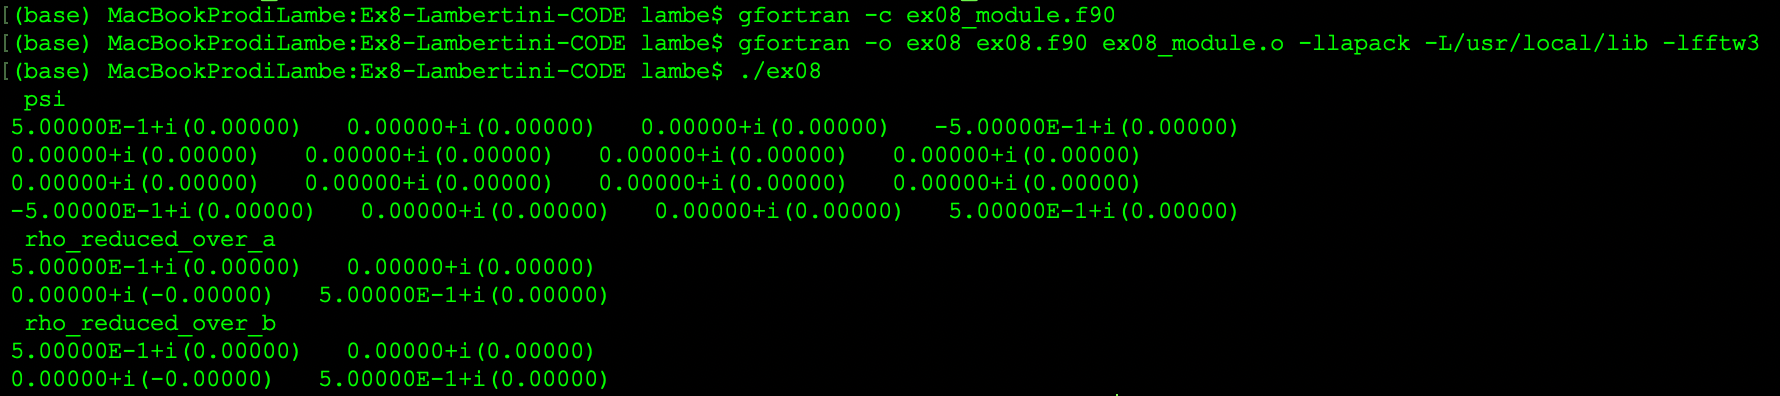
\includegraphics[width=.85\textwidth]{output}\hfill
%    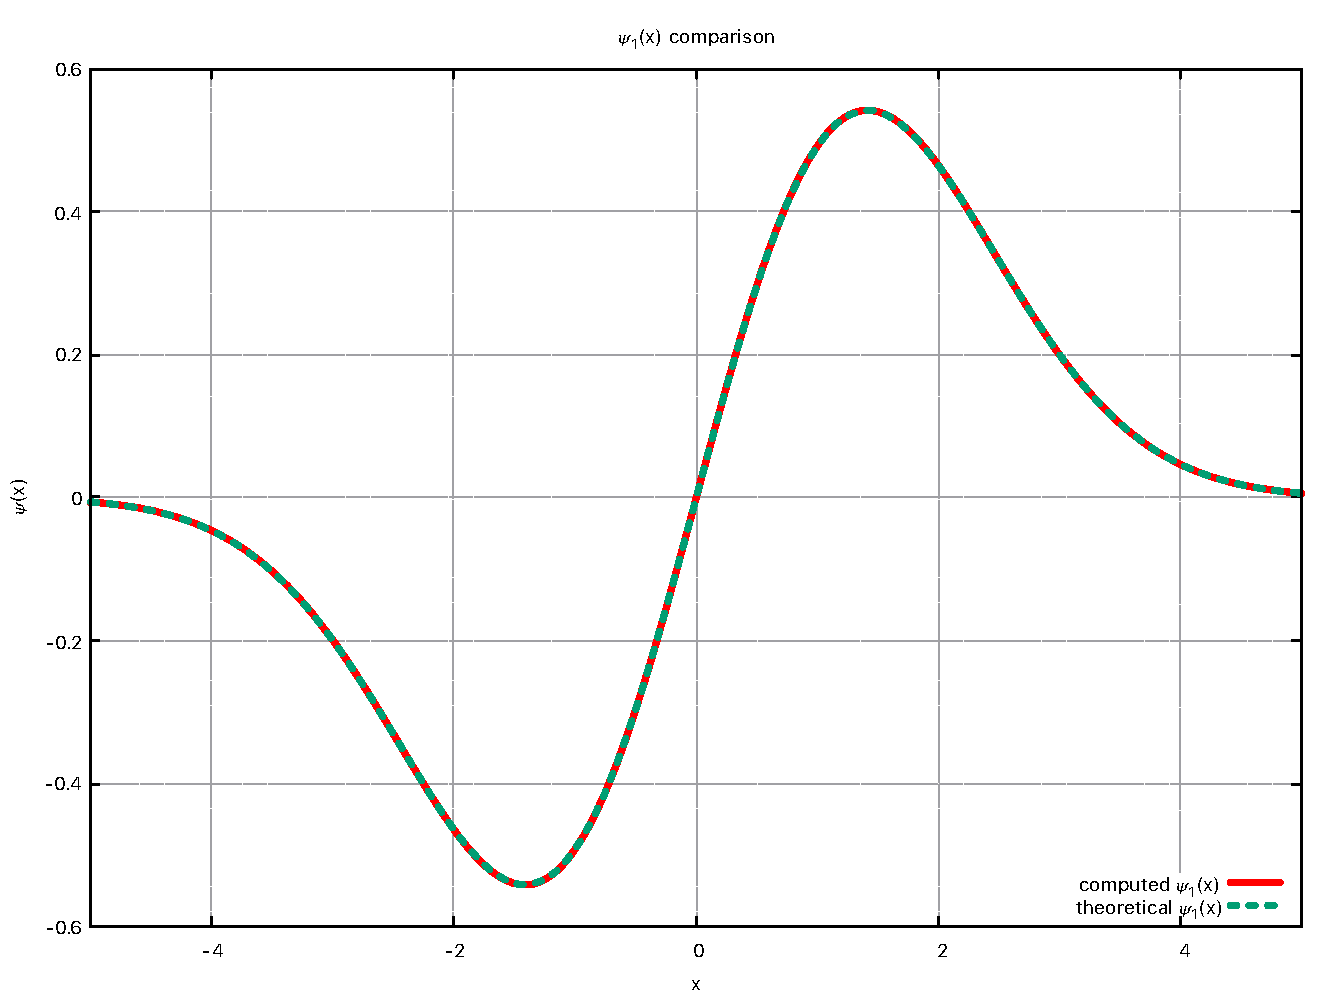
\includegraphics[width=.45\textwidth]{psi_1}\hfill
%    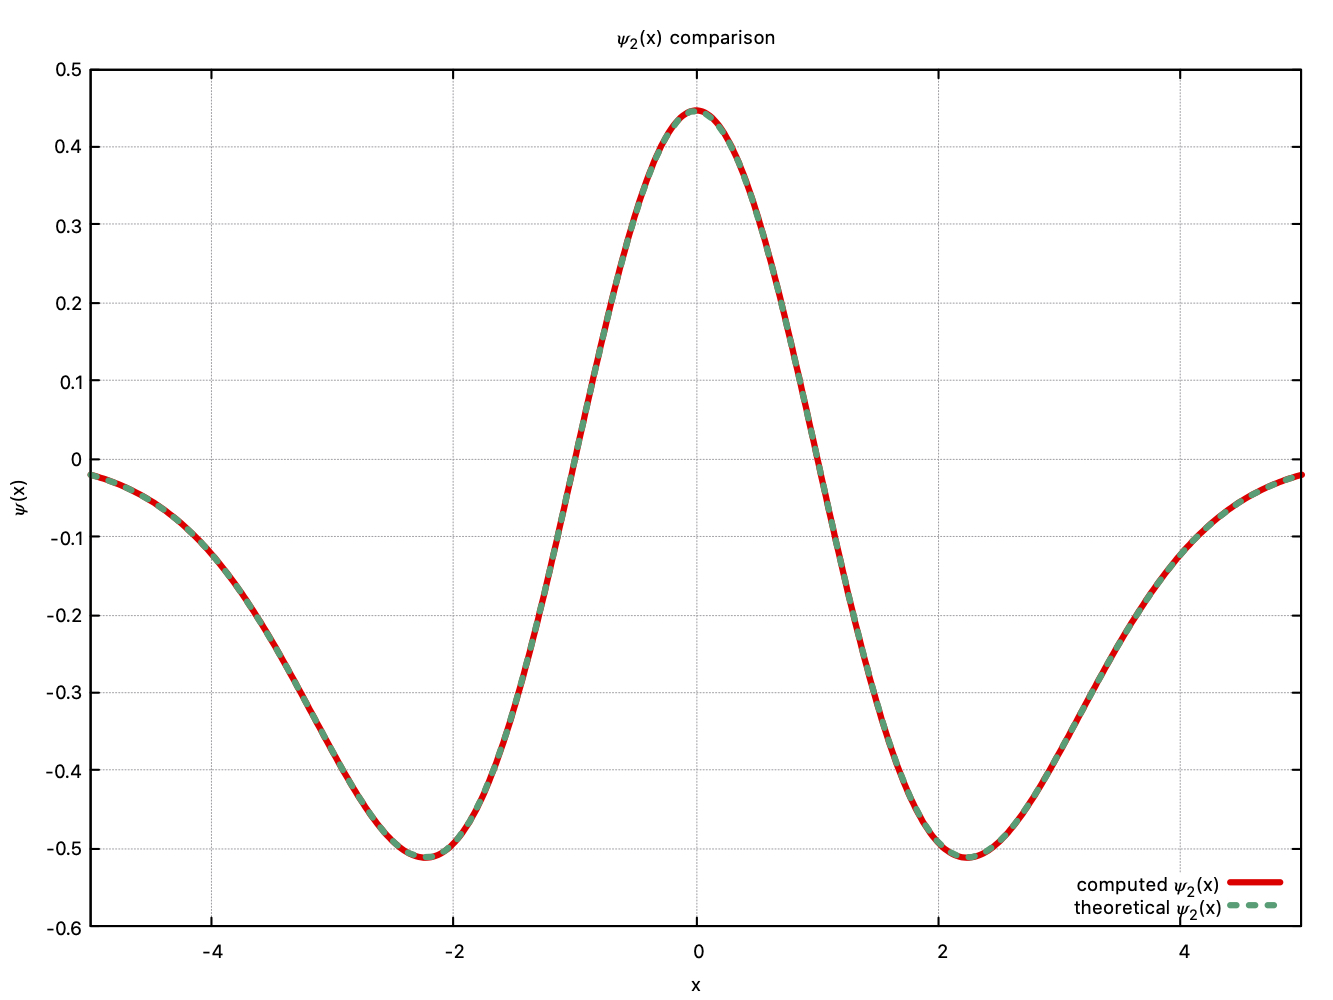
\includegraphics[width=.45\textwidth]{psi_2}
%%    \\[\smallskipamount]
%%    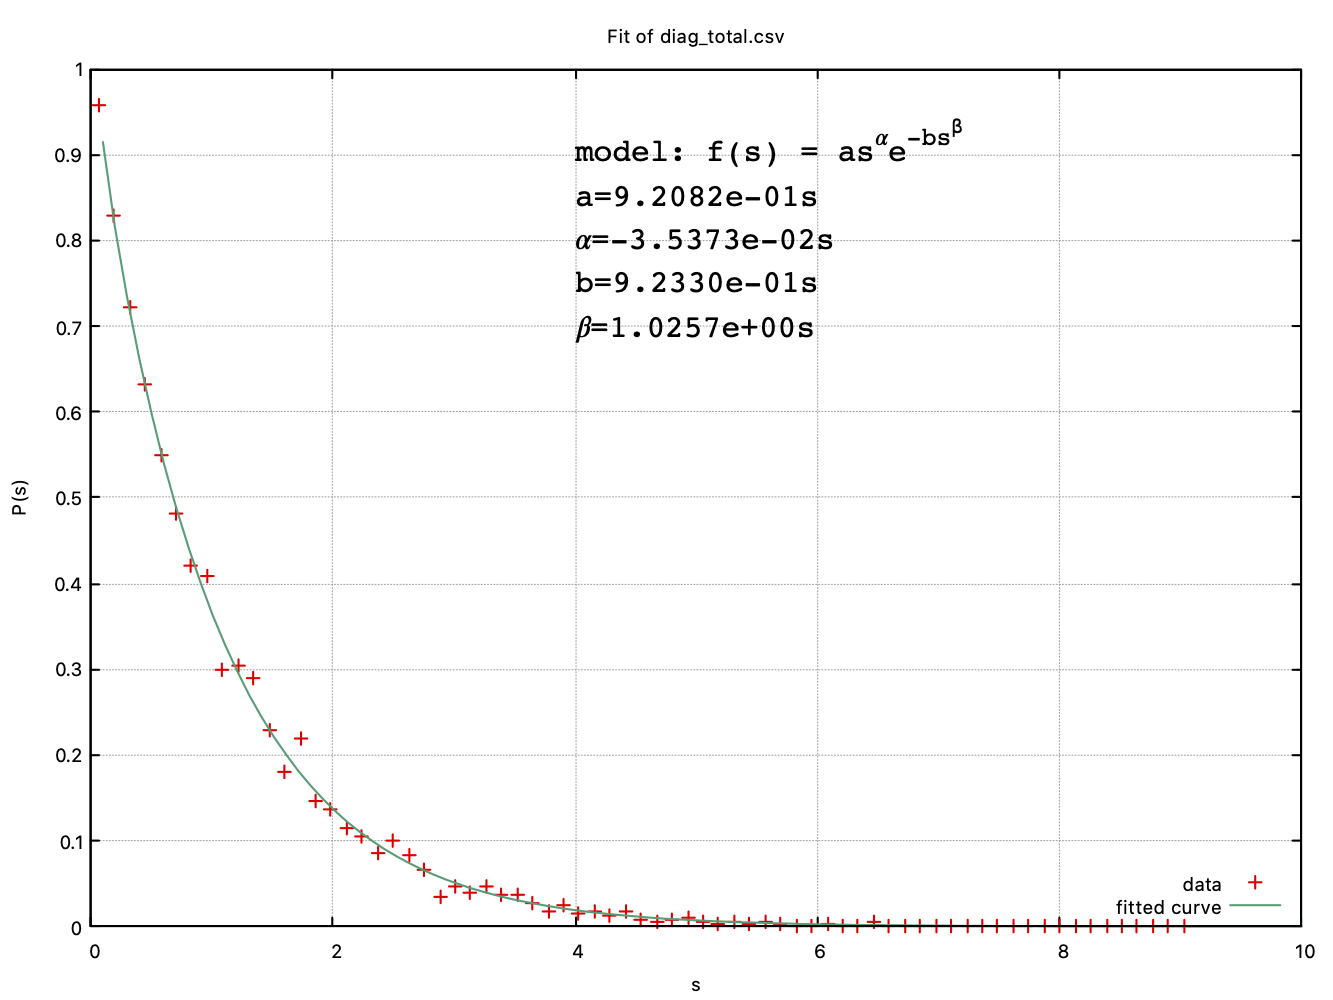
\includegraphics[width=.33\textwidth]{diag_total}\hfill
%%    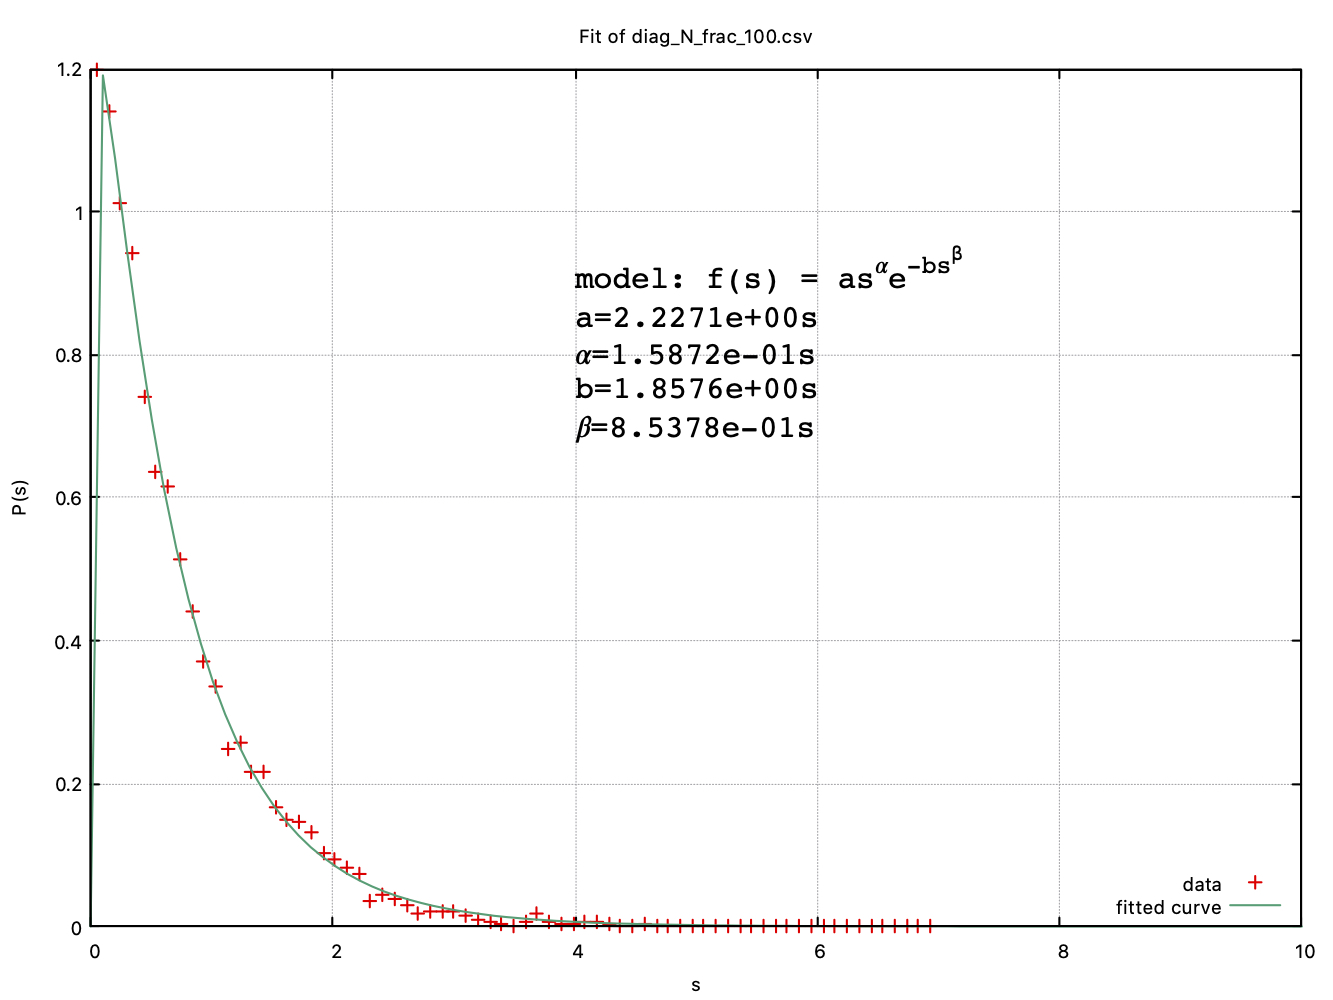
\includegraphics[width=.33\textwidth]{diag_N_frac_100}\hfill
%%    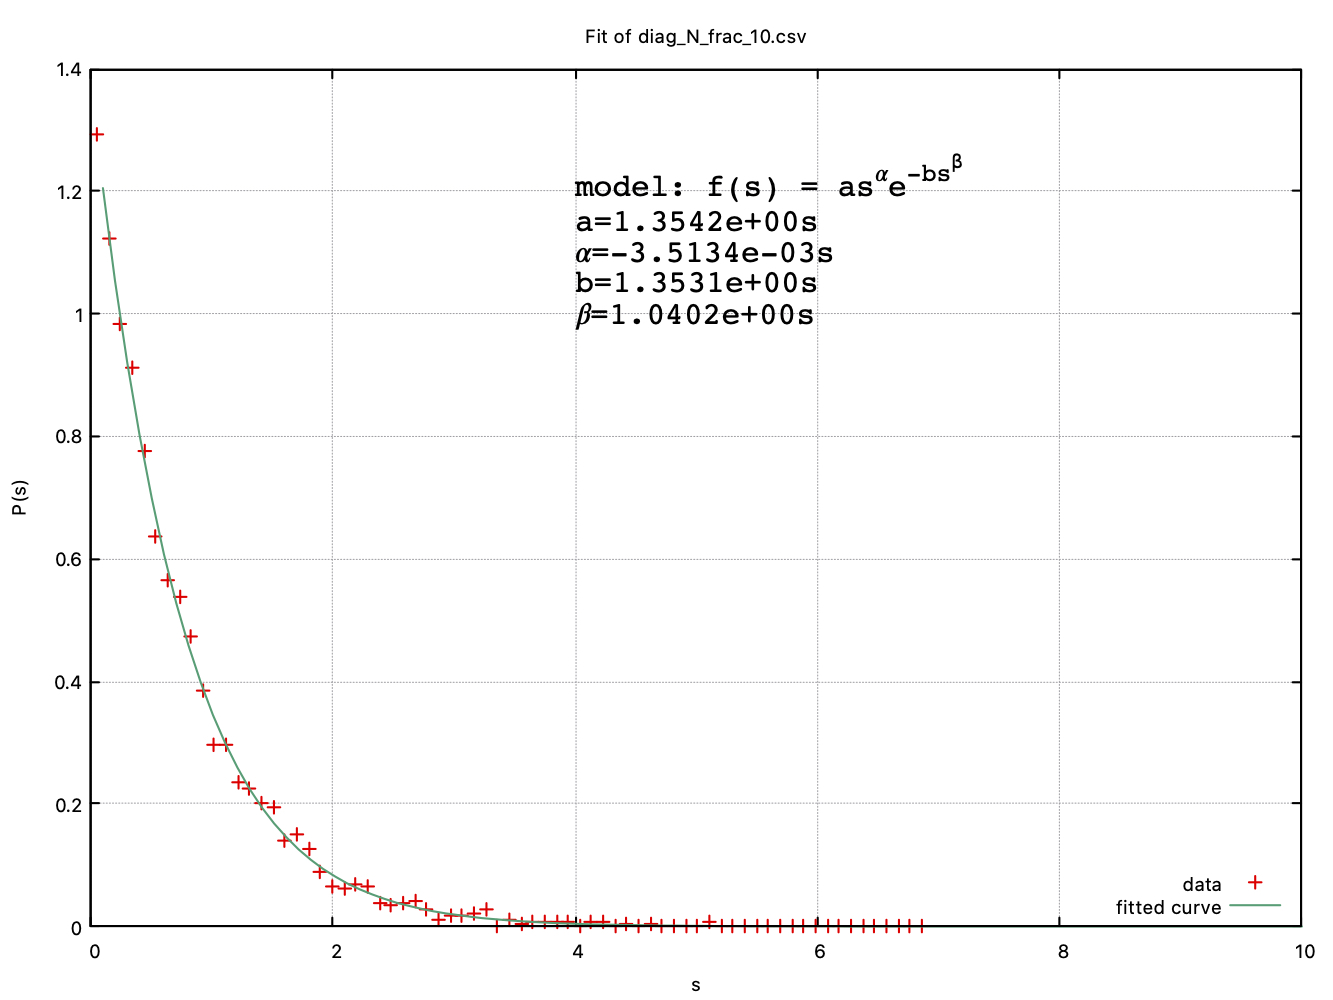
\includegraphics[width=.33\textwidth]{diag_N_frac_10}
    \caption{Output of the program \textit{ex08.f90}}\label{fig:foobar}
\end{figure}
We can see that the results are coherent with what expected from theory.

\section{Self-evaluation}
I think the main objectives of the exercise are reached. I have learnt how to implement tensor operations in Fortran in the quantum-mechanical framework. I'm aware that the report is not rich enough of details and explanations but I have not had much time this week, I hope that the work is still sufficient.



\end{document}
